\documentclass[9pt, aspectratio=169]{beamer}
% \documentclass[10pt]{beamer}
\usepackage[utf8]{inputenc}
\usepackage[T1]{fontenc}
\usepackage[english]{babel}
\usetheme{Frankfurt}

\usepackage[backend=biber, style=authoryear]{biblatex}
\addbibresource{local_references.bib}

%\usepackage{lmodern}
\usepackage{amsfonts,amssymb,amsmath}
\usepackage[english]{babel}
\usetheme{Frankfurt}

\usepackage{csquotes}
\usepackage{setspace}

\usepackage{colortbl}
\usepackage{tabularx}
\renewcommand\tabularxcolumn[1]{m{#1}}

% --- Tickz
\usepackage{physics}
\usepackage{amsmath}
\usepackage{tikz}
\usepackage{mathdots}
\usepackage{yhmath}
\usepackage{cancel}
\usepackage{color}
\usepackage{siunitx}
\usepackage{array}
\usepackage{multirow}
\usepackage{amssymb}
\usepackage{gensymb}
\usepackage{tabularx}
\usepackage{extarrows}
\usepackage{booktabs}
\usetikzlibrary{fadings}
\usetikzlibrary{patterns}
\usetikzlibrary{shadows.blur}
\usetikzlibrary{shapes}

% ---------

\usepackage{booktabs}
\usepackage{setspace}
\usepackage{amssymb}
\usepackage{adjustbox}
\usepackage{pifont}
\usepackage[inkscapeformat=png]{svg}
\usepackage{graphicx}
\usepackage{times}
\setbeamertemplate{caption}[numbered]
% % \setbeamertemplate{bibliography item}{[\theenumiv]}

\setbeamerfont{bibliography item}{size=\tiny}
\setbeamerfont{bibliography entry author}{size=\tiny}
\setbeamerfont{bibliography entry title}{size=\tiny}
\setbeamerfont{bibliography entry location}{size=\tiny}
\setbeamerfont{bibliography entry note}{size=\tiny}

\setbeamerfont{frametitle}{size=\large}

\usepackage{caption}
\usepackage{float}
\usepackage{xcolor}
\usepackage{listings}
\usepackage{animate}

\definecolor{codegreen}{rgb}{0,0.6,0}
\definecolor{codegray}{rgb}{0.5,0.5,0.5}
\definecolor{codepurple}{rgb}{0.58,0,0.82}
\definecolor{backcolour}{rgb}{0.95,0.95,0.92}
 
\lstdefinestyle{mystyle}{
    backgroundcolor=\color{backcolour},   
    commentstyle=\color{codegreen},
    keywordstyle=\color{magenta},
    numberstyle=\tiny\color{codegray},
    stringstyle=\color{codepurple},
    basicstyle=\footnotesize,
    breakatwhitespace=false,         
    breaklines=true,                 
    captionpos=b,                    
    keepspaces=true,                 
    numbers=left,                    
    numbersep=5pt,                  
    showspaces=false,                
    showstringspaces=false,
    showtabs=false,                  
    tabsize=2
}
 
\lstset{style=mystyle}

\usepackage{ragged2e}
\setbeamercolor{section in foot}{fg=white,bg=darkorange}
\setbeamercolor{subsection in foot}{fg=white,bg=darkorange}
\setbeamercolor{frametitle}{fg=white, bg=darkorange}
\setbeamercolor{title}{fg=white, bg=darkorange}
\setbeamercolor{frame}{bg=darkorange}
\setbeamercolor{block title}{bg=darkorange,fg=white}

\setbeamercolor{item}{fg=darkorange}

% \definecolor{darkorange}{rgb}{0.81, 0.52, 0.05}
\definecolor{darkorange}{rgb}{1,0.5,0}
\definecolor{darkorange2}{rgb}{1, 0.64, 0.2}
\definecolor{honeydew}{rgb}{1, 0.85, 0.45}


\newenvironment{variableblock}[3]{%
  \setbeamercolor{block body}{#2}
  \setbeamercolor{block title}{#3}
  \begin{block}{#1}}{\end{block}}

\newenvironment{prosblock}[1]{%
  % \setbeamercolor{block body}{bg=blue,fg=white}
  \setbeamercolor{block title}{bg=blue,fg=white}
  \begin{block}{#1}}{\end{block}}

\newenvironment{consblock}[1]{%
  % \setbeamercolor{block body}{bg=red,fg=white}
  \setbeamercolor{block title}{bg=red,fg=white}
  \begin{block}{#1}}{\end{block}}

\newcommand{\cmark}{\ding{51}}%
\newcommand{\xmark}{\ding{55}}%

\renewcommand{\arraystretch}{1.5}

% Please add the following required packages to your document preamble:
\usepackage{booktabs}
\usepackage{multirow}
\usepackage{colortbl}
% Beamer presentation requires \usepackage{colortbl} instead of \usepackage[table,xcdraw]{xcolor}

\usepackage{tabularray}\UseTblrLibrary{varwidth}
\usepackage{xcolor}
\def\BibTeX{{\rm B\kern-.05em{\sc i\kern-.025em b}\kern-.08em
    T\kern-.1667em\lower.7ex\hbox{E}\kern-.125emX}}
% \usepackage{cite}
\usepackage{amsmath}
\newcommand{\probP}{\text{I\kern-0.15em P}}
\usepackage{etoolbox}
\patchcmd{\thebibliography}{\section*{\refname}}{}{}{}

\setlength\tabcolsep{0.5pt}

\renewcommand{\arraystretch}{0.9}
\setlength{\tabcolsep}{2pt}

\usepackage{pgffor}

\setbeamerfont{bibliography item}{size=\tiny}
\setbeamerfont{bibliography entry author}{size=\tiny}
\setbeamerfont{bibliography entry title}{size=\tiny}
\setbeamerfont{bibliography entry location}{size=\tiny}
\setbeamerfont{bibliography entry note}{size=\tiny}

\setbeamerfont{bibliography entry author}{shape=\upshape,series=\mdseries,size=\footnotesize}
\setbeamerfont{bibliography entry title}{shape=\slshape,series=\mdseries,size=\footnotesize}
\setbeamerfont{bibliography entry journal}{shape=\upshape,series=\mdseries,size=\footnotesize}
\setbeamerfont{bibliography entry note}{shape=\upshape,series=\mdseries,size=\footnotesize}

\renewcommand*{\bibfont}{\scriptsize}

\newenvironment<>{varblock}[2][.9\textwidth]{%
  \setlength{\textwidth}{#1}
  \begin{actionenv}#3%
    \def\insertblocktitle{#2}%
    \par%
    \usebeamertemplate{block begin}}
  {\par%
    \usebeamertemplate{block end}%
  \end{actionenv}}

% \setbeamertemplate{footline}[frame number]

\setbeamertemplate{footline}{
  \leavevmode%
  \hfill
  \usebeamercolor[fg]{page number in head/foot}%
  \scriptsize%
  \ifnum\value{framenumber}>19%
    Appendix \number\numexpr\value{framenumber}-19\relax/32%
  \else%
    \ifnum\value{framenumber}>16%
      %
    \else
      \number\numexpr\value{framenumber}\relax/16%
    \fi

  \fi%
  \hspace{1em}
}


\begin{document}

\author{\textbf{Julien Soulé}, Jean-Paul Jamont, Michel Occello, Paul Théron, Louis-Marie Traonouez}

\title{\textbf{Towards a Multi-Agent Simulation of Cyber-attackers and Cyber-defenders Battles}}

\subtitle{SMC 2023 Presentation}

% \logo{
\includegraphics[scale=0.01]{figures/grenoble-inp_logo.png}}

\institute{\footnotesize \textit{University Grenoble Alpes, Grenoble
INP, LCIS, 26000, Valence, France \\
julien.soule@lcis.grenoble-inp.fr}}

\date{\textit{\footnotesize \today}}

%\subject{}
\setbeamercovered{transparent}
%\setbeamertemplate{navigation symbols}{}
\begin{frame}[plain]
	\maketitle\vspace{-0.8cm}
	\begin{figure}[ht!]
		\centering
            
\includegraphics[height=0.8cm]{figures/la-ruche_logo.png}
            \hspace{0.8cm}
            
\includegraphics[height=0.8cm]{figures/lcis_logo.png}
            \hspace{0.8cm}
		
\includegraphics[height=0.8cm]{figures/grenoble-inp_logo.png}
            \hspace{0.8cm}
            
\includegraphics[height=0.8cm]{figures/uga_logo.jpg}
	\end{figure}
\end{frame}

% \begin{frame}{Content}
%   \tableofcontents
% \end{frame}

\addtocounter{framenumber}{-1}

\begin{frame}{Objectifs de la journée}

  \begin{itemize}
    \item Faire un point sur le sujet de la thèse et les travaux effectués
    \item Faire le point sur l'état d'avancement du manuscrit
    \item Faire le point sur le planning jusqu'à la fin de la thèse
  \end{itemize}

\end{frame}

\begin{frame}{Plan de la journée}
  \tableofcontents
\end{frame}

\section{Aperçu / Retour sur Thèse \& Travaux}

\begin{frame}{Contexte}

  \begin{itemize}
    \item Explosion de l'IoT, hétérogenité \& faible protection des objets connectés \\ $\rightarrow$ augmentation de la surface d'attaque difficilement pris en compte
    \item Attaques décentralisé et stratégisé en combinant différents vecteurs d'attaques par différentes entités \\ $\rightarrow$ peu couverts par systèmes de cyberdéfense actuels
    \item Montée en autonomie des différents attaquants par l'utilisation de bots ou assistance reposant sur l'IA \\ $\rightarrow$ renforce difficulté à assurer cyberdéfense
  \end{itemize}
\end{frame}

\begin{frame}{Motivation}
  \begin{itemize}
    \item Besoin assurer cyberdéfense adaptée au contexte de déploiement, des attaques/menaces cyber de façon dynamique \\ $\rightarrow$ apprentissage \& adaptation
    \item Besoin de  prendre en compte le systèmes distribués et décentralisés \\ $\rightarrow$ exclure approche centralisée
    \item Besoin de prendre en compte exigences de conception particulières \\ $\rightarrow$ interaction/controle opérateurs
    \item Besoin prise en compte décentralisation et distribution des cyber-attaques \\ $\rightarrow$ privilegier cyber-défense de multiple vecteurs d'action collaboratifs
    \item Travaux initiés par l'IST-152 puis l'AICA IWG sur les agents AICA \\
          $\rightarrow$ agent AICA couvre la plupart des besoins mais manque aspect distribué et décentralisé \\
          $\rightarrow$ Approche d'un SMA flexible et auto-organisé d'un agent AICA
  \end{itemize}
\end{frame}

\begin{frame}{Question de recherche}

  \begin{block}{Question de recherche}
    \begin{itemize}
      \item[Q1] Comment automatiser la conception d’un SMA de cyberdéfense auto-organisé capable d’atteindre de manière optimale et continue dans le temps ses objectifs de cyberdéfense dans un environnement dynamique, en tenant compte :
            \begin{itemize}
              \item des contraintes dynamiques liées à l'environnement incluant les cyber-attaques ;
              \item et des exigences architecturales définies par le cadre AICA ?
            \end{itemize}
    \end{itemize}
  \end{block}

\end{frame}

\begin{frame}{Verrous théoriques et techniques}

  \begin{itemize}
    \item[G1] Pas de formalisation du problème de conception d'un SMA de Cyberdéfense
    \item[G2] Faible généralisabilité et automatisation des approches de conception de SMA, et inexistence pour les SMA de Cyberdéfense
    \item[G3] Peu d'adaptivité dans la réponse cyber vis à vis des contraintes dynamiques de l'environnement et des cyber-attaques
    \item[G4] Faible explicabilité des SMA émergents (peu explicite, pas de vision organisationnelle)
    \item[G5] Impossibilité ou risques liés à l'experimentation directe sur l'environnement réel durant la conception du SMA
  \end{itemize}

\end{frame}

\begin{frame}{Hypothèses}

  \begin{itemize}
    \item[H1] Question de recherche peut être formalisé comme problème d'optimisation des politiques des agents sous contraintes de l'environnement (incluant attaquants) et exigences de conception pour maximiser objectif ;
    \item[H2] Techniques "World Models" peut permettre modéliser environnement déploiement comme simulation en plus de modélisation manuelle ;
    \item[H3] Techniques "MARL" peut permettre de résoudre le problème formalisé automatiquement ;
    \item[H4] Contraintes des exigences de conception, peuvent être intégrées dans le processus MARL pour guider/contraindre l'apprentissage des agents en utilisant un modèle organisationnel explicite
    \item[H5] Comportements des agents peuvent être compris dans un modèle organisationnel explicite
  \end{itemize}

\end{frame}

\begin{frame}{Aperçu de la réponse générale proposée}

  \begin{itemize}
    \item En général : Passer d'une approche \textquote{IA Symbolique} à une approche plus orientée \textquote{IA Machine Learning - MARL/RL} pour implémenter l'auto-organisation ;
    \item \textbf{MOISE+MARL Assisted MAS Design (MAMAD)} : Une méthode de conception en \textbf{4 phases séquentielle} sur un \textbf{cycle fermé}
    \item Chaque phase se base sur des contributions reposant sur les hypothèses précédentes
          \begin{itemize}
            \item \textbf{Modélisation} : utilisation des "World Models" pour créer un modèle de simulation réaliste
            \item \textbf{Entrainement} : utilisation de MARL + modèle organisationnel $\mathcal{M}OISE^+$ $\rightarrow$ entrainer les agents dans le cadre d'une organisation
            \item \textbf{Analyse} : utilisation de "Unsupervised Learning" sur trajectoires + modèle organisationnel $\mathcal{M}OISE^+$ $\rightarrow$ voir les agents dans le cadre d'une organisation
            \item \textbf{Transfert} : utilisation d'un framework Kubernetes pour le déploiement / mise à jour des politiques des agents dans l'environnement de déploiement ; et amélioration fidélité du modèle simulé à la réalité
          \end{itemize}
  \end{itemize}

\end{frame}

\begin{frame}{Aperçu de la réponse générale proposée}

  \begin{columns}[c]

    \hspace{-1.5cm}

    \begin{column}{0.5\textwidth}
      \begin{enumerate}
        \item Modéliser l’environnement à partir de traces réelles, de l’objectif global et des exigences de conception, sous forme de rôles et d’objectifs ;
        \item Entraînement des agents à l’aide de MOISE+MARL ;
        \item Analyse pour inférrer des rôles et objectifs émergents des agents $\rightarrow$ amélioration des spécifications organisationnelles appliquées ($\times$ itérations 2-3) ;
        \item Transferer les politiques pour piloter les actionneurs des agents (déploiement direct ou à distance) + génère nouvelles traces $\rightarrow$ modèle simulé plus fidèle.
      \end{enumerate}

    \end{column}

    \hspace{-1.5cm}

    \begin{column}{0.5\textwidth}
      \begin{figure}[h!]
        \centering
        


\tikzset{every picture/.style={line width=0.75pt}} %set default line width to 0.75pt        

\begin{tikzpicture}[x=0.75pt,y=0.75pt,yscale=-1,xscale=1]
%uncomment if require: \path (0,3307); %set diagram left start at 0, and has height of 3307

%Shape: Smiley Face [id:dp29065495216725257] 
\draw  [line width=1.5]  (85.38,2800.11) .. controls (85.38,2797.7) and (87.16,2795.75) .. (89.36,2795.75) .. controls (91.55,2795.75) and (93.34,2797.7) .. (93.34,2800.11) .. controls (93.34,2802.52) and (91.55,2804.48) .. (89.36,2804.48) .. controls (87.16,2804.48) and (85.38,2802.52) .. (85.38,2800.11) -- cycle ; \draw  [line width=1.5]  (87.61,2798.63) .. controls (87.61,2798.39) and (87.78,2798.19) .. (88,2798.19) .. controls (88.22,2798.19) and (88.4,2798.39) .. (88.4,2798.63) .. controls (88.4,2798.87) and (88.22,2799.07) .. (88,2799.07) .. controls (87.78,2799.07) and (87.61,2798.87) .. (87.61,2798.63) -- cycle ; \draw  [line width=1.5]  (90.31,2798.63) .. controls (90.31,2798.39) and (90.49,2798.19) .. (90.71,2798.19) .. controls (90.93,2798.19) and (91.11,2798.39) .. (91.11,2798.63) .. controls (91.11,2798.87) and (90.93,2799.07) .. (90.71,2799.07) .. controls (90.49,2799.07) and (90.31,2798.87) .. (90.31,2798.63) -- cycle ; \draw  [line width=1.5]  (87.37,2801.86) .. controls (88.69,2803.02) and (90.02,2803.02) .. (91.35,2801.86) ;
%Shape: Rectangle [id:dp42672371521059915] 
\draw  [dash pattern={on 5.63pt off 4.5pt}][line width=1.5]  (74.03,2763.75) -- (192,2763.75) -- (192,2813.93) -- (74.03,2813.93) -- cycle ;
%Shape: Smiley Face [id:dp9817389082285293] 
\draw  [line width=1.5]  (144.45,2803.6) .. controls (144.45,2801.19) and (146.24,2799.24) .. (148.43,2799.24) .. controls (150.63,2799.24) and (152.41,2801.19) .. (152.41,2803.6) .. controls (152.41,2806.01) and (150.63,2807.97) .. (148.43,2807.97) .. controls (146.24,2807.97) and (144.45,2806.01) .. (144.45,2803.6) -- cycle ; \draw  [line width=1.5]  (146.68,2802.12) .. controls (146.68,2801.88) and (146.86,2801.68) .. (147.08,2801.68) .. controls (147.3,2801.68) and (147.48,2801.88) .. (147.48,2802.12) .. controls (147.48,2802.36) and (147.3,2802.56) .. (147.08,2802.56) .. controls (146.86,2802.56) and (146.68,2802.36) .. (146.68,2802.12) -- cycle ; \draw  [line width=1.5]  (149.39,2802.12) .. controls (149.39,2801.88) and (149.57,2801.68) .. (149.79,2801.68) .. controls (150.01,2801.68) and (150.18,2801.88) .. (150.18,2802.12) .. controls (150.18,2802.36) and (150.01,2802.56) .. (149.79,2802.56) .. controls (149.57,2802.56) and (149.39,2802.36) .. (149.39,2802.12) -- cycle ; \draw  [line width=1.5]  (146.44,2805.35) .. controls (147.77,2806.51) and (149.1,2806.51) .. (150.42,2805.35) ;
%Shape: Smiley Face [id:dp49419175504212776] 
\draw  [line width=1.5]  (179.09,2781.5) .. controls (179.09,2779.09) and (180.87,2777.13) .. (183.06,2777.13) .. controls (185.26,2777.13) and (187.04,2779.09) .. (187.04,2781.5) .. controls (187.04,2783.91) and (185.26,2785.86) .. (183.06,2785.86) .. controls (180.87,2785.86) and (179.09,2783.91) .. (179.09,2781.5) -- cycle ; \draw  [line width=1.5]  (181.31,2780.01) .. controls (181.31,2779.77) and (181.49,2779.58) .. (181.71,2779.58) .. controls (181.93,2779.58) and (182.11,2779.77) .. (182.11,2780.01) .. controls (182.11,2780.25) and (181.93,2780.45) .. (181.71,2780.45) .. controls (181.49,2780.45) and (181.31,2780.25) .. (181.31,2780.01) -- cycle ; \draw  [line width=1.5]  (184.02,2780.01) .. controls (184.02,2779.77) and (184.2,2779.58) .. (184.42,2779.58) .. controls (184.64,2779.58) and (184.81,2779.77) .. (184.81,2780.01) .. controls (184.81,2780.25) and (184.64,2780.45) .. (184.42,2780.45) .. controls (184.2,2780.45) and (184.02,2780.25) .. (184.02,2780.01) -- cycle ; \draw  [line width=1.5]  (181.07,2783.24) .. controls (182.4,2784.4) and (183.73,2784.4) .. (185.05,2783.24) ;
%Flowchart: Punched Tape [id:dp3565745198144521] 
\draw  [fill={rgb, 255:red, 255; green, 255; blue, 255 }  ,fill opacity=1 ] (291.67,2877.34) .. controls (291.67,2880.23) and (301.36,2882.58) .. (313.31,2882.58) .. controls (325.26,2882.58) and (334.95,2880.23) .. (334.95,2877.34) .. controls (334.95,2874.45) and (344.64,2872.11) .. (356.6,2872.11) .. controls (368.55,2872.11) and (378.24,2874.45) .. (378.24,2877.34) -- (378.24,2919.23) .. controls (378.24,2916.34) and (368.55,2913.99) .. (356.6,2913.99) .. controls (344.64,2913.99) and (334.95,2916.34) .. (334.95,2919.23) .. controls (334.95,2922.12) and (325.26,2924.46) .. (313.31,2924.46) .. controls (301.36,2924.46) and (291.67,2922.12) .. (291.67,2919.23) -- cycle ;
%Straight Lines [id:da23451091058783402] 
\draw [line width=1.5]    (320.63,2891.89) -- (349.47,2889.91) ;
\draw [shift={(352.46,2889.7)}, rotate = 176.08] [color={rgb, 255:red, 0; green, 0; blue, 0 }  ][line width=1.5]    (8.53,-2.57) .. controls (5.42,-1.09) and (2.58,-0.23) .. (0,0) .. controls (2.58,0.23) and (5.42,1.09) .. (8.53,2.57)   ;
%Straight Lines [id:da05993633349010663] 
\draw [line width=1.5]    (320.63,2894.07) -- (335.84,2901.48) ;
\draw [shift={(338.53,2902.79)}, rotate = 205.98] [color={rgb, 255:red, 0; green, 0; blue, 0 }  ][line width=1.5]    (8.53,-2.57) .. controls (5.42,-1.09) and (2.58,-0.23) .. (0,0) .. controls (2.58,0.23) and (5.42,1.09) .. (8.53,2.57)   ;
%Shape: Smiley Face [id:dp5316832937595011] 
\draw  [line width=1.5]  (312.91,2893.34) .. controls (312.91,2890.93) and (314.69,2888.98) .. (316.89,2888.98) .. controls (319.09,2888.98) and (320.87,2890.93) .. (320.87,2893.34) .. controls (320.87,2895.75) and (319.09,2897.7) .. (316.89,2897.7) .. controls (314.69,2897.7) and (312.91,2895.75) .. (312.91,2893.34) -- cycle ; \draw  [line width=1.5]  (315.14,2891.86) .. controls (315.14,2891.61) and (315.32,2891.42) .. (315.54,2891.42) .. controls (315.76,2891.42) and (315.94,2891.61) .. (315.94,2891.86) .. controls (315.94,2892.1) and (315.76,2892.29) .. (315.54,2892.29) .. controls (315.32,2892.29) and (315.14,2892.1) .. (315.14,2891.86) -- cycle ; \draw  [line width=1.5]  (317.85,2891.86) .. controls (317.85,2891.61) and (318.02,2891.42) .. (318.24,2891.42) .. controls (318.46,2891.42) and (318.64,2891.61) .. (318.64,2891.86) .. controls (318.64,2892.1) and (318.46,2892.29) .. (318.24,2892.29) .. controls (318.02,2892.29) and (317.85,2892.1) .. (317.85,2891.86) -- cycle ; \draw  [line width=1.5]  (314.9,2895.08) .. controls (316.23,2896.25) and (317.55,2896.25) .. (318.88,2895.08) ;
%Shape: Smiley Face [id:dp5491508300746957] 
\draw  [line width=1.5]  (338.38,2904.97) .. controls (338.38,2902.56) and (340.16,2900.61) .. (342.35,2900.61) .. controls (344.55,2900.61) and (346.33,2902.56) .. (346.33,2904.97) .. controls (346.33,2907.38) and (344.55,2909.34) .. (342.35,2909.34) .. controls (340.16,2909.34) and (338.38,2907.38) .. (338.38,2904.97) -- cycle ; \draw  [line width=1.5]  (340.6,2903.49) .. controls (340.6,2903.25) and (340.78,2903.05) .. (341,2903.05) .. controls (341.22,2903.05) and (341.4,2903.25) .. (341.4,2903.49) .. controls (341.4,2903.73) and (341.22,2903.93) .. (341,2903.93) .. controls (340.78,2903.93) and (340.6,2903.73) .. (340.6,2903.49) -- cycle ; \draw  [line width=1.5]  (343.31,2903.49) .. controls (343.31,2903.25) and (343.49,2903.05) .. (343.71,2903.05) .. controls (343.93,2903.05) and (344.1,2903.25) .. (344.1,2903.49) .. controls (344.1,2903.73) and (343.93,2903.93) .. (343.71,2903.93) .. controls (343.49,2903.93) and (343.31,2903.73) .. (343.31,2903.49) -- cycle ; \draw  [line width=1.5]  (340.36,2906.72) .. controls (341.69,2907.88) and (343.02,2907.88) .. (344.34,2906.72) ;
%Shape: Smiley Face [id:dp21362593128550156] 
\draw  [line width=1.5]  (352.64,2888.69) .. controls (352.64,2886.28) and (354.42,2884.32) .. (356.61,2884.32) .. controls (358.81,2884.32) and (360.59,2886.28) .. (360.59,2888.69) .. controls (360.59,2891.1) and (358.81,2893.05) .. (356.61,2893.05) .. controls (354.42,2893.05) and (352.64,2891.1) .. (352.64,2888.69) -- cycle ; \draw  [line width=1.5]  (354.86,2887.2) .. controls (354.86,2886.96) and (355.04,2886.77) .. (355.26,2886.77) .. controls (355.48,2886.77) and (355.66,2886.96) .. (355.66,2887.2) .. controls (355.66,2887.44) and (355.48,2887.64) .. (355.26,2887.64) .. controls (355.04,2887.64) and (354.86,2887.44) .. (354.86,2887.2) -- cycle ; \draw  [line width=1.5]  (357.57,2887.2) .. controls (357.57,2886.96) and (357.75,2886.77) .. (357.97,2886.77) .. controls (358.19,2886.77) and (358.36,2886.96) .. (358.36,2887.2) .. controls (358.36,2887.44) and (358.19,2887.64) .. (357.97,2887.64) .. controls (357.75,2887.64) and (357.57,2887.44) .. (357.57,2887.2) -- cycle ; \draw  [line width=1.5]  (354.62,2890.43) .. controls (355.95,2891.59) and (357.28,2891.59) .. (358.6,2890.43) ;
%Left Arrow [id:dp22187584774212898] 
\draw   (215,2804.55) -- (220.28,2802) -- (220.28,2803.27) -- (263.54,2803.27) -- (263.54,2805.82) -- (220.28,2805.82) -- (220.28,2807.09) -- cycle ;
%Left Arrow [id:dp1861077704673879] 
\draw   (315.35,2834) -- (317.89,2837.8) -- (316.62,2837.8) -- (316.62,2868.91) -- (314.07,2868.91) -- (314.07,2837.8) -- (312.8,2837.8) -- cycle ;
%Left Arrow [id:dp2590948740182193] 
\draw   (130.55,2868.91) -- (128,2865.11) -- (129.27,2865.11) -- (129.27,2834) -- (131.82,2834) -- (131.82,2865.11) -- (133.09,2865.11) -- cycle ;
%Left Arrow [id:dp7631269314674067] 
\draw   (262.54,2900.55) -- (257.26,2903.09) -- (257.26,2901.82) -- (214,2901.82) -- (214,2899.27) -- (257.26,2899.27) -- (257.26,2898) -- cycle ;
%Shape: Arc [id:dp8010751146858193] 
\draw  [draw opacity=0] (78.55,2898.86) .. controls (77.97,2897.43) and (79.7,2895.07) .. (82.41,2893.59) .. controls (85.13,2892.11) and (87.81,2892.08) .. (88.39,2893.51) -- (83.47,2896.19) -- cycle ; \draw   (78.55,2898.86) .. controls (77.97,2897.43) and (79.7,2895.07) .. (82.41,2893.59) .. controls (85.13,2892.11) and (87.81,2892.08) .. (88.39,2893.51) ;  
%Shape: Arc [id:dp2168479262754166] 
\draw  [draw opacity=0] (79.96,2900.21) .. controls (79.37,2898.78) and (80.79,2896.59) .. (83.12,2895.32) .. controls (85.45,2894.06) and (87.81,2894.19) .. (88.39,2895.63) -- (84.17,2897.92) -- cycle ; \draw   (79.96,2900.21) .. controls (79.37,2898.78) and (80.79,2896.59) .. (83.12,2895.32) .. controls (85.45,2894.06) and (87.81,2894.19) .. (88.39,2895.63) ;  
%Shape: Arc [id:dp1657064934185728] 
\draw  [draw opacity=0] (81.36,2901.56) .. controls (81.36,2901.56) and (81.36,2901.56) .. (81.36,2901.56) .. controls (80.78,2900.13) and (81.88,2898.11) .. (83.82,2897.06) .. controls (85.76,2896) and (87.81,2896.31) .. (88.39,2897.74) -- (84.88,2899.65) -- cycle ; \draw   (81.36,2901.56) .. controls (81.36,2901.56) and (81.36,2901.56) .. (81.36,2901.56) .. controls (80.78,2900.13) and (81.88,2898.11) .. (83.82,2897.06) .. controls (85.76,2896) and (87.81,2896.31) .. (88.39,2897.74) ;  
%Shape: Arc [id:dp6696163073703636] 
\draw  [draw opacity=0] (82.77,2902.92) .. controls (82.77,2902.92) and (82.77,2902.92) .. (82.77,2902.92) .. controls (82.77,2902.92) and (82.77,2902.92) .. (82.77,2902.92) .. controls (82.19,2901.48) and (82.97,2899.63) .. (84.53,2898.79) .. controls (86.08,2897.94) and (87.81,2898.42) .. (88.39,2899.86) -- (85.58,2901.39) -- cycle ; \draw   (82.77,2902.92) .. controls (82.77,2902.92) and (82.77,2902.92) .. (82.77,2902.92) .. controls (82.77,2902.92) and (82.77,2902.92) .. (82.77,2902.92) .. controls (82.19,2901.48) and (82.97,2899.63) .. (84.53,2898.79) .. controls (86.08,2897.94) and (87.81,2898.42) .. (88.39,2899.86) ;  
%Shape: Arc [id:dp5914598807756752] 
\draw  [draw opacity=0] (84.18,2904.27) .. controls (83.6,2902.83) and (84.07,2901.15) .. (85.23,2900.52) .. controls (86.4,2899.89) and (87.81,2900.54) .. (88.4,2901.97) -- (86.29,2903.12) -- cycle ; \draw   (84.18,2904.27) .. controls (83.6,2902.83) and (84.07,2901.15) .. (85.23,2900.52) .. controls (86.4,2899.89) and (87.81,2900.54) .. (88.4,2901.97) ;  

%Image [id:dp3722282424817167] 
\draw (291.67,2795.75) node  {
\includegraphics[width=7.64pt,height=13.09pt]{figures/robot.png}};
%Shape: Rectangle [id:dp9197785817800539] 
\draw  [line width=1.5]  (275.37,2763.75) -- (390.8,2763.75) -- (390.8,2813.93) -- (275.37,2813.93) -- cycle ;
%Image [id:dp9715658782589778] 
\draw (382.32,2779.46) node  {
\includegraphics[width=7.64pt,height=13.09pt]{figures/robot.png}};
%Image [id:dp635616861971029] 
\draw (352.78,2801.57) node  {
\includegraphics[width=7.64pt,height=13.09pt]{figures/robot.png}};
%Shape: Rectangle [id:dp647928357040308] 
\draw  [fill={rgb, 255:red, 0; green, 0; blue, 0 }  ,fill opacity=1 ] (291.67,2769.57) -- (301.85,2769.57) -- (301.85,2781.21) -- (291.67,2781.21) -- cycle ;
%Shape: Rectangle [id:dp9626828362725837] 
\draw  [fill={rgb, 255:red, 0; green, 0; blue, 0 }  ,fill opacity=1 ] (373.15,2792.84) -- (383.33,2792.84) -- (383.33,2804.48) -- (373.15,2804.48) -- cycle ;
%Shape: Ellipse [id:dp6171740062199291] 
\draw  [fill={rgb, 255:red, 0; green, 0; blue, 0 }  ,fill opacity=1 ] (347.69,2775.39) .. controls (347.69,2772.17) and (349.97,2769.57) .. (352.78,2769.57) .. controls (355.59,2769.57) and (357.87,2772.17) .. (357.87,2775.39) .. controls (357.87,2778.6) and (355.59,2781.21) .. (352.78,2781.21) .. controls (349.97,2781.21) and (347.69,2778.6) .. (347.69,2775.39) -- cycle ;
%Shape: Triangle [id:dp8145134127966778] 
\draw  [fill={rgb, 255:red, 0; green, 0; blue, 0 }  ,fill opacity=1 ] (322.22,2792.84) -- (327.31,2804.48) -- (317.13,2804.48) -- cycle ;
%Shape: Rectangle [id:dp07981685971419106] 
\draw  [fill={rgb, 255:red, 0; green, 0; blue, 0 }  ,fill opacity=1 ] (89.45,2769.57) -- (99.64,2769.57) -- (99.64,2781.21) -- (89.45,2781.21) -- cycle ;
%Shape: Rectangle [id:dp9786998324005067] 
\draw  [fill={rgb, 255:red, 0; green, 0; blue, 0 }  ,fill opacity=1 ] (170.94,2792.84) -- (181.12,2792.84) -- (181.12,2804.48) -- (170.94,2804.48) -- cycle ;
%Shape: Ellipse [id:dp6465785854464419] 
\draw  [fill={rgb, 255:red, 0; green, 0; blue, 0 }  ,fill opacity=1 ] (145.47,2775.39) .. controls (145.47,2772.17) and (147.75,2769.57) .. (150.57,2769.57) .. controls (153.38,2769.57) and (155.66,2772.17) .. (155.66,2775.39) .. controls (155.66,2778.6) and (153.38,2781.21) .. (150.57,2781.21) .. controls (147.75,2781.21) and (145.47,2778.6) .. (145.47,2775.39) -- cycle ;
%Shape: Triangle [id:dp5909890868954251] 
\draw  [fill={rgb, 255:red, 0; green, 0; blue, 0 }  ,fill opacity=1 ] (120.01,2792.84) -- (125.1,2804.48) -- (114.92,2804.48) -- cycle ;
%Shape: Smiley Face [id:dp661163164093121] 
\draw  [line width=1.5]  (85.52,2909.38) .. controls (85.52,2906.98) and (87.3,2905.03) .. (89.5,2905.03) .. controls (91.7,2905.03) and (93.48,2906.98) .. (93.48,2909.38) .. controls (93.48,2911.78) and (91.7,2913.73) .. (89.5,2913.73) .. controls (87.3,2913.73) and (85.52,2911.78) .. (85.52,2909.38) -- cycle ; \draw  [line width=1.5]  (87.75,2907.9) .. controls (87.75,2907.66) and (87.93,2907.46) .. (88.15,2907.46) .. controls (88.37,2907.46) and (88.55,2907.66) .. (88.55,2907.9) .. controls (88.55,2908.14) and (88.37,2908.33) .. (88.15,2908.33) .. controls (87.93,2908.33) and (87.75,2908.14) .. (87.75,2907.9) -- cycle ; \draw  [line width=1.5]  (90.46,2907.9) .. controls (90.46,2907.66) and (90.63,2907.46) .. (90.85,2907.46) .. controls (91.07,2907.46) and (91.25,2907.66) .. (91.25,2907.9) .. controls (91.25,2908.14) and (91.07,2908.33) .. (90.85,2908.33) .. controls (90.63,2908.33) and (90.46,2908.14) .. (90.46,2907.9) -- cycle ; \draw  [line width=1.5]  (87.51,2911.12) .. controls (88.84,2912.28) and (90.16,2912.28) .. (91.49,2911.12) ;
%Shape: Rectangle [id:dp9256921796782376] 
\draw  [dash pattern={on 5.63pt off 4.5pt}][line width=1.5]  (74.17,2873.12) -- (192,2873.12) -- (192,2923.15) -- (74.17,2923.15) -- cycle ;
%Shape: Smiley Face [id:dp12230401154700177] 
\draw  [line width=1.5]  (144.6,2912.86) .. controls (144.6,2910.46) and (146.38,2908.51) .. (148.58,2908.51) .. controls (150.77,2908.51) and (152.56,2910.46) .. (152.56,2912.86) .. controls (152.56,2915.26) and (150.77,2917.21) .. (148.58,2917.21) .. controls (146.38,2917.21) and (144.6,2915.26) .. (144.6,2912.86) -- cycle ; \draw  [line width=1.5]  (146.83,2911.38) .. controls (146.83,2911.14) and (147,2910.94) .. (147.22,2910.94) .. controls (147.44,2910.94) and (147.62,2911.14) .. (147.62,2911.38) .. controls (147.62,2911.62) and (147.44,2911.81) .. (147.22,2911.81) .. controls (147,2911.81) and (146.83,2911.62) .. (146.83,2911.38) -- cycle ; \draw  [line width=1.5]  (149.53,2911.38) .. controls (149.53,2911.14) and (149.71,2910.94) .. (149.93,2910.94) .. controls (150.15,2910.94) and (150.33,2911.14) .. (150.33,2911.38) .. controls (150.33,2911.62) and (150.15,2911.81) .. (149.93,2911.81) .. controls (149.71,2911.81) and (149.53,2911.62) .. (149.53,2911.38) -- cycle ; \draw  [line width=1.5]  (146.59,2914.6) .. controls (147.91,2915.76) and (149.24,2915.76) .. (150.57,2914.6) ;
%Shape: Smiley Face [id:dp8847243900502049] 
\draw  [line width=1.5]  (179.23,2890.23) .. controls (179.23,2887.83) and (181.01,2885.88) .. (183.21,2885.88) .. controls (185.4,2885.88) and (187.19,2887.83) .. (187.19,2890.23) .. controls (187.19,2892.63) and (185.4,2894.58) .. (183.21,2894.58) .. controls (181.01,2894.58) and (179.23,2892.63) .. (179.23,2890.23) -- cycle ; \draw  [line width=1.5]  (181.46,2888.75) .. controls (181.46,2888.51) and (181.63,2888.32) .. (181.85,2888.32) .. controls (182.07,2888.32) and (182.25,2888.51) .. (182.25,2888.75) .. controls (182.25,2888.99) and (182.07,2889.19) .. (181.85,2889.19) .. controls (181.63,2889.19) and (181.46,2888.99) .. (181.46,2888.75) -- cycle ; \draw  [line width=1.5]  (184.16,2888.75) .. controls (184.16,2888.51) and (184.34,2888.32) .. (184.56,2888.32) .. controls (184.78,2888.32) and (184.96,2888.51) .. (184.96,2888.75) .. controls (184.96,2888.99) and (184.78,2889.19) .. (184.56,2889.19) .. controls (184.34,2889.19) and (184.16,2888.99) .. (184.16,2888.75) -- cycle ; \draw  [line width=1.5]  (181.22,2891.97) .. controls (182.54,2893.13) and (183.87,2893.13) .. (185.2,2891.97) ;
%Shape: Rectangle [id:dp5525291488755686] 
\draw  [fill={rgb, 255:red, 0; green, 0; blue, 0 }  ,fill opacity=1 ] (89.6,2878.92) -- (99.78,2878.92) -- (99.78,2890.53) -- (89.6,2890.53) -- cycle ;
%Shape: Rectangle [id:dp35042622253694655] 
\draw  [fill={rgb, 255:red, 0; green, 0; blue, 0 }  ,fill opacity=1 ] (171.08,2902.13) -- (181.27,2902.13) -- (181.27,2913.73) -- (171.08,2913.73) -- cycle ;
%Shape: Ellipse [id:dp9658079314838142] 
\draw  [fill={rgb, 255:red, 0; green, 0; blue, 0 }  ,fill opacity=1 ] (145.62,2884.72) .. controls (145.62,2881.52) and (147.9,2878.92) .. (150.71,2878.92) .. controls (153.52,2878.92) and (155.8,2881.52) .. (155.8,2884.72) .. controls (155.8,2887.93) and (153.52,2890.53) .. (150.71,2890.53) .. controls (147.9,2890.53) and (145.62,2887.93) .. (145.62,2884.72) -- cycle ;
%Shape: Triangle [id:dp5926435260290868] 
\draw  [fill={rgb, 255:red, 0; green, 0; blue, 0 }  ,fill opacity=1 ] (120.15,2902.13) -- (125.25,2913.73) -- (115.06,2913.73) -- cycle ;
%Shape: Arc [id:dp2058241396036773] 
\draw  [draw opacity=0] (133.56,2911.66) .. controls (132.26,2911.1) and (132.06,2908.03) .. (133.1,2904.81) .. controls (134.15,2901.58) and (136.04,2899.43) .. (137.34,2899.99) -- (135.45,2905.83) -- cycle ; \draw   (133.56,2911.66) .. controls (132.26,2911.1) and (132.06,2908.03) .. (133.1,2904.81) .. controls (134.15,2901.58) and (136.04,2899.43) .. (137.34,2899.99) ;  
%Shape: Arc [id:dp9303770446429336] 
\draw  [draw opacity=0] (135.39,2911.51) .. controls (135.39,2911.51) and (135.39,2911.51) .. (135.39,2911.51) .. controls (135.39,2911.51) and (135.39,2911.51) .. (135.39,2911.51) .. controls (134.1,2910.95) and (133.77,2908.25) .. (134.67,2905.49) .. controls (135.56,2902.72) and (137.34,2900.94) .. (138.63,2901.5) -- (137.01,2906.51) -- cycle ; \draw   (135.39,2911.51) .. controls (135.39,2911.51) and (135.39,2911.51) .. (135.39,2911.51) .. controls (135.39,2911.51) and (135.39,2911.51) .. (135.39,2911.51) .. controls (134.1,2910.95) and (133.77,2908.25) .. (134.67,2905.49) .. controls (135.56,2902.72) and (137.34,2900.94) .. (138.63,2901.5) ;  
%Shape: Arc [id:dp23450230368676772] 
\draw  [draw opacity=0] (137.22,2911.35) .. controls (137.22,2911.35) and (137.22,2911.35) .. (137.22,2911.35) .. controls (137.22,2911.35) and (137.22,2911.35) .. (137.22,2911.35) .. controls (135.93,2910.79) and (135.48,2908.47) .. (136.23,2906.17) .. controls (136.98,2903.86) and (138.63,2902.45) .. (139.93,2903.02) -- (138.58,2907.19) -- cycle ; \draw   (137.22,2911.35) .. controls (137.22,2911.35) and (137.22,2911.35) .. (137.22,2911.35) .. controls (137.22,2911.35) and (137.22,2911.35) .. (137.22,2911.35) .. controls (135.93,2910.79) and (135.48,2908.47) .. (136.23,2906.17) .. controls (136.98,2903.86) and (138.63,2902.45) .. (139.93,2903.02) ;  
%Shape: Arc [id:dp32480365085094887] 
\draw  [draw opacity=0] (139.06,2911.2) .. controls (139.06,2911.2) and (139.06,2911.2) .. (139.06,2911.2) .. controls (137.76,2910.64) and (137.2,2908.69) .. (137.79,2906.85) .. controls (138.39,2905) and (139.92,2903.97) .. (141.22,2904.53) -- (140.14,2907.87) -- cycle ; \draw   (139.06,2911.2) .. controls (139.06,2911.2) and (139.06,2911.2) .. (139.06,2911.2) .. controls (137.76,2910.64) and (137.2,2908.69) .. (137.79,2906.85) .. controls (138.39,2905) and (139.92,2903.97) .. (141.22,2904.53) ;  
%Shape: Arc [id:dp7108436649867611] 
\draw  [draw opacity=0] (140.89,2911.05) .. controls (139.6,2910.48) and (138.91,2908.91) .. (139.36,2907.53) .. controls (139.8,2906.14) and (141.22,2905.48) .. (142.51,2906.05) -- (141.7,2908.55) -- cycle ; \draw   (140.89,2911.05) .. controls (139.6,2910.48) and (138.91,2908.91) .. (139.36,2907.53) .. controls (139.8,2906.14) and (141.22,2905.48) .. (142.51,2906.05) ;  

%Shape: Arc [id:dp7234198948762418] 
\draw  [draw opacity=0] (171.31,2898) .. controls (171.31,2898) and (171.31,2898) .. (171.31,2898) .. controls (169.93,2898.17) and (168.53,2895.53) .. (168.19,2892.12) .. controls (167.85,2888.7) and (168.7,2885.8) .. (170.08,2885.64) .. controls (170.08,2885.64) and (170.08,2885.64) .. (170.08,2885.64) -- (170.69,2891.82) -- cycle ; \draw   (171.31,2898) .. controls (171.31,2898) and (171.31,2898) .. (171.31,2898) .. controls (169.93,2898.17) and (168.53,2895.53) .. (168.19,2892.12) .. controls (167.85,2888.7) and (168.7,2885.8) .. (170.08,2885.64) .. controls (170.08,2885.64) and (170.08,2885.64) .. (170.08,2885.64) ;  
%Shape: Arc [id:dp05399242918401237] 
\draw  [draw opacity=0] (172.88,2896.92) .. controls (172.88,2896.92) and (172.88,2896.92) .. (172.88,2896.92) .. controls (171.5,2897.09) and (170.15,2894.85) .. (169.86,2891.92) .. controls (169.57,2888.99) and (170.45,2886.49) .. (171.83,2886.32) -- (172.35,2891.62) -- cycle ; \draw   (172.88,2896.92) .. controls (172.88,2896.92) and (172.88,2896.92) .. (172.88,2896.92) .. controls (171.5,2897.09) and (170.15,2894.85) .. (169.86,2891.92) .. controls (169.57,2888.99) and (170.45,2886.49) .. (171.83,2886.32) ;  
%Shape: Arc [id:dp7827225311205266] 
\draw  [draw opacity=0] (174.46,2895.84) .. controls (174.46,2895.84) and (174.46,2895.84) .. (174.46,2895.84) .. controls (173.08,2896) and (171.76,2894.16) .. (171.52,2891.72) .. controls (171.28,2889.28) and (172.2,2887.17) .. (173.58,2887.01) -- (174.02,2891.42) -- cycle ; \draw   (174.46,2895.84) .. controls (174.46,2895.84) and (174.46,2895.84) .. (174.46,2895.84) .. controls (173.08,2896) and (171.76,2894.16) .. (171.52,2891.72) .. controls (171.28,2889.28) and (172.2,2887.17) .. (173.58,2887.01) ;  
%Shape: Arc [id:dp9906438850599013] 
\draw  [draw opacity=0] (176.03,2894.76) .. controls (174.65,2894.92) and (173.38,2893.47) .. (173.19,2891.52) .. controls (172.99,2889.57) and (173.95,2887.86) .. (175.33,2887.69) -- (175.68,2891.23) -- cycle ; \draw   (176.03,2894.76) .. controls (174.65,2894.92) and (173.38,2893.47) .. (173.19,2891.52) .. controls (172.99,2889.57) and (173.95,2887.86) .. (175.33,2887.69) ;  
%Shape: Arc [id:dp545106976508444] 
\draw  [draw opacity=0] (177.61,2893.68) .. controls (177.61,2893.68) and (177.61,2893.68) .. (177.61,2893.68) .. controls (176.23,2893.84) and (174.99,2892.79) .. (174.85,2891.33) .. controls (174.7,2889.86) and (175.7,2888.54) .. (177.08,2888.38) -- (177.34,2891.03) -- cycle ; \draw   (177.61,2893.68) .. controls (177.61,2893.68) and (177.61,2893.68) .. (177.61,2893.68) .. controls (176.23,2893.84) and (174.99,2892.79) .. (174.85,2891.33) .. controls (174.7,2889.86) and (175.7,2888.54) .. (177.08,2888.38) ;  

%Down Arrow [id:dp8971518008111754] 
\draw   (230,2776) -- (232.5,2776) -- (232.5,2764) -- (237.5,2764) -- (237.5,2776) -- (240,2776) -- (235,2784) -- cycle ;


% Text Node
\draw (187.23,2773.35) node  [font=\scriptsize] [align=left] {\begin{minipage}[lt]{8.67pt}\setlength\topsep{0pt}
\begin{center}
{\footnotesize \textbf{\textcolor[rgb]{0.82,0.01,0.11}{?}}}
\end{center}

\end{minipage}};
% Text Node
\draw (152.6,2795.46) node  [font=\scriptsize] [align=left] {\begin{minipage}[lt]{8.67pt}\setlength\topsep{0pt}
\begin{center}
{\footnotesize \textbf{\textcolor[rgb]{0.82,0.01,0.11}{?}}}
\end{center}

\end{minipage}};
% Text Node
\draw (93.53,2791.97) node  [font=\scriptsize] [align=left] {\begin{minipage}[lt]{8.67pt}\setlength\topsep{0pt}
\begin{center}
{\footnotesize \textbf{\textcolor[rgb]{0.82,0.01,0.11}{?}}}
\end{center}

\end{minipage}};
% Text Node
\draw (182.5,2877.5) node  [font=\scriptsize] [align=left] {\begin{minipage}[lt]{8.67pt}\setlength\topsep{0pt}
\begin{center}
{\footnotesize $\displaystyle \mathbf{\textcolor[rgb]{0.82,0.01,0.11}{\pi }\textcolor[rgb]{0.82,0.01,0.11}{_{3}}}$}
\end{center}

\end{minipage}};
% Text Node
\draw (97.6,2901.34) node  [font=\scriptsize] [align=left] {\begin{minipage}[lt]{8.67pt}\setlength\topsep{0pt}
\begin{center}
{\footnotesize $\displaystyle \mathbf{\textcolor[rgb]{0.82,0.01,0.11}{\pi }\textcolor[rgb]{0.82,0.01,0.11}{_{1}}}$}
\end{center}

\end{minipage}};
% Text Node
\draw (358.3,2787.5) node  [font=\scriptsize] [align=left] {\begin{minipage}[lt]{8.67pt}\setlength\topsep{0pt}
\begin{center}
{\footnotesize $\displaystyle \textcolor[rgb]{0.82,0.01,0.11}{(}\mathbf{\textcolor[rgb]{0.82,0.01,0.11}{\pi }\textcolor[rgb]{0.82,0.01,0.11}{_{2}}}\textcolor[rgb]{0.82,0.01,0.11}{)}$}
\end{center}

\end{minipage}};
% Text Node
\draw (368.3,2770.5) node  [font=\scriptsize] [align=left] {\begin{minipage}[lt]{8.67pt}\setlength\topsep{0pt}
\begin{center}
{\footnotesize $\displaystyle \textcolor[rgb]{0.82,0.01,0.11}{(}\mathbf{\textcolor[rgb]{0.82,0.01,0.11}{\pi }\textcolor[rgb]{0.82,0.01,0.11}{_{3}}}\textcolor[rgb]{0.82,0.01,0.11}{)}$}
\end{center}

\end{minipage}};
% Text Node
\draw (299.81,2787.31) node  [font=\scriptsize] [align=left] {\begin{minipage}[lt]{8.67pt}\setlength\topsep{0pt}
\begin{center}
{\footnotesize $\displaystyle \textcolor[rgb]{0.82,0.01,0.11}{(}\mathbf{\textcolor[rgb]{0.82,0.01,0.11}{\pi }\textcolor[rgb]{0.82,0.01,0.11}{_{1}}}\textcolor[rgb]{0.82,0.01,0.11}{)}$}
\end{center}

\end{minipage}};
% Text Node
\draw (154.64,2902.5) node  [font=\scriptsize] [align=left] {\begin{minipage}[lt]{8.67pt}\setlength\topsep{0pt}
\begin{center}
{\footnotesize $\displaystyle \mathbf{\textcolor[rgb]{0.82,0.01,0.11}{\pi }\textcolor[rgb]{0.82,0.01,0.11}{_{2}}}$}
\end{center}

\end{minipage}};
% Text Node
\draw (336.27,2821.93) node  [font=\footnotesize] [align=left] {\begin{minipage}[lt]{83.6pt}\setlength\topsep{0pt}
\begin{center}
\textit{Target environment}
\end{center}

\end{minipage}};
% Text Node
\draw (336,2940) node   [align=left] {\begin{minipage}[lt]{62.53pt}\setlength\topsep{0pt}
\begin{center}
\textit{{\footnotesize "blueprints" of}\\{\footnotesize suggested MAS}}
\end{center}

\end{minipage}};
% Text Node
\draw (139.36,2940.19) node   [align=left] {\begin{minipage}[lt]{96.97pt}\setlength\topsep{0pt}
\begin{center}
\textit{{\footnotesize Simulated environment + Trained agents}}
\end{center}

\end{minipage}};
% Text Node
\draw (138.5,2824.5) node  [font=\footnotesize] [align=left] {\begin{minipage}[lt]{93.02pt}\setlength\topsep{0pt}
\begin{center}
\textit{Simulated environment}
\end{center}

\end{minipage}};
% Text Node
\draw (171.5,2848.5) node  [font=\footnotesize] [align=left] {\textbf{2) Training}};
% Text Node
\draw (357.3,2848.5) node  [font=\footnotesize] [align=left] {\textbf{4) Transfer}};
% Text Node
\draw (348.3,2877.5) node  [font=\scriptsize] [align=left] {\begin{minipage}[lt]{8.67pt}\setlength\topsep{0pt}
\begin{center}
{\footnotesize $\displaystyle \mathbf{\textcolor[rgb]{0.82,0.01,0.11}{\pi }\textcolor[rgb]{0.82,0.01,0.11}{_{3}}}$}
\end{center}

\end{minipage}};
% Text Node
\draw (354.3,2900.5) node  [font=\scriptsize] [align=left] {\begin{minipage}[lt]{8.67pt}\setlength\topsep{0pt}
\begin{center}
{\footnotesize $\displaystyle \mathbf{\textcolor[rgb]{0.82,0.01,0.11}{\pi }\textcolor[rgb]{0.82,0.01,0.11}{_{2}}}$}
\end{center}

\end{minipage}};
% Text Node
\draw (305.3,2886.5) node  [font=\scriptsize] [align=left] {\begin{minipage}[lt]{8.67pt}\setlength\topsep{0pt}
\begin{center}
{\footnotesize $\displaystyle \mathbf{\textcolor[rgb]{0.82,0.01,0.11}{\pi }\textcolor[rgb]{0.82,0.01,0.11}{_{1}}}$}
\end{center}

\end{minipage}};
% Text Node
\draw (236.43,2889.27) node  [font=\footnotesize] [align=left] {\textbf{3) Analyze}};
% Text Node
\draw (233.5,2792.5) node  [font=\footnotesize] [align=left] {\textbf{1) Modeling}};


\end{tikzpicture}
        \caption{Cycle de vie d’un SMA conçu avec MAMAD}
        \label{fig:cycle}
      \end{figure}
    \end{column}
  \end{columns}


\end{frame}

\section{Détails des contributions par article}

\begin{frame}{Organisation des contributions}

  \begin{itemize}
    \item Chaque article de conférence présente une ou plusieurs des contributions s'intégrant dans la réponse générale proposée et peuvent se superposer en partie entre elles ;
    \item Chaque article de conférence évalue ces contributions sur un ou plusieurs cas d'application spécifique ;
    \item L'article de journal présente la méthode qui orchestre toute ces contributions comme réponse, voulue comme complète, de la question de recherche
  \end{itemize}

  \

  \begin{center}
    \begin{table}[h!]
      \begin{tabular}{ c c c c c c c }
        \textbf{Article}                   & \multicolumn{2}{c}{\textbf{Modélisation}} & \multicolumn{2}{c}{\textbf{Entrainement}} & \textbf{Analyse} & \textbf{Transfert}                         \\
        \cmidrule(lr){2-3} \cmidrule(lr){4-5}
                                           & Manuel                                    & Automatisé                                & Vanilla          & Contraint          &           &           \\
        \midrule                                                                                                                                                                                   \\
        SMC                                & \ding{51}                                 & \ding{55}                                 & \ding{51}        & \ding{55}          & \ding{55} & \ding{55} \\
        AIAI                               & \ding{51}                                 & \ding{55}                                 & \ding{55}        & $\sim$             & $\sim$    & \ding{55} \\
        $\text{CAID}_{\lnot \text{pub.}}$  & \ding{51}                                 & \ding{55}                                 & \ding{55}        & \ding{51}          & \ding{55} & \ding{55} \\
        $\text{PRIMA}_{\lnot \text{pub.}}$ & \ding{51}                                 & \ding{55}                                 & \ding{55}        & \ding{51}          & $\sim$    & $\sim$    \\
        AAMAS                              & \ding{55}                                 & \ding{55}                                 & \ding{55}        & \ding{51}          & \ding{51} & \ding{55} \\
        CLOUD                              & \ding{55}                                 & \ding{51}                                 & \ding{55}        & \ding{51}          & \ding{51} & \ding{51} \\
        Journal                            & \ding{51}                                 & \ding{51}                                 & \ding{51}        & \ding{51}          & \ding{51} & \ding{51}
      \end{tabular}
      \caption{Couverture des contributions de la méthode MAMAD (journal) par les articles de conférence}
    \end{table}
  \end{center}

\end{frame}

\begin{frame}{Assisting Multi-Agent System Design with
    MOISE+ and MARL: The MAMAD Method (\textbf{Journal})}
  Voir journal + corrections
\end{frame}

\begin{frame}{Towards a Multi-Agent Simulation of Cyber-attackers and Cyber-defenders Battles (\textbf{SMC})}
  Voir papier + présentation
\end{frame}

\begin{frame}{A MARL-Based Approach for Easing MAS Organization Engineering (\textbf{AIAI})}
  Voir papier + présentation
\end{frame}

\begin{frame}{An organizationally-oriented approach to enhancing explainability and control in multi-agent reinforcement learning (\textbf{AAMAS})}
  Voir papier + présentation
\end{frame}


\begin{frame}{An Organization-oriented MARL Approach for Cyberdefense in a Drone Swarm Scenario (\textbf{CAID})}
  Voir papier
\end{frame}

\begin{frame}{Streamlining Resilient Kubernetes Autoscaling with Multi-Agent Systems via an Automated Online Design Framework (\textbf{CLOUD})}
  Voir papier
\end{frame}

\section{Planning thèse}
\begin{frame}{Planning thèse}

  \begin{itemize}
    \item Juin
          \begin{itemize}
            \item Finaliser le manuscrit (fin Juin)
          \end{itemize}
    \item Juillet
          \begin{itemize}
            \item Envoyer première version
          \end{itemize}
    \item Août
          \begin{itemize}
            \item Rien
          \end{itemize}
    \item Septembre
          \begin{itemize}
            \item Retours, prise en compte remarques
            \item Entrainement oral pour défense (fin Septembre)
          \end{itemize}
    \item Octobre
          \begin{itemize}
            \item Entrainement oral pour défense (début Octobre)
            \item Défense (mi-Octobre)
          \end{itemize}
  \end{itemize}

\end{frame}

\section{Manuscrit}

\begin{frame}{Des articles au manuscrit}
  \begin{itemize}
    \item En général : Le journal sur la méthode MAMAD donne la structure générale de la contribution pour répondre à la question de recherche $\rightarrow$ Chapitre \textbf{Méthode de conception d'un SMA de Cyberdéfense}
    \item Les articles de conf sont des cas d'application particuliers $\rightarrow$ Chapitre \textbf{Experimentation et évaluation}
  \end{itemize}
\end{frame}

\begin{frame}[allowframebreaks]{Plan}

  \begin{enumerate}

    \item Introduction
          \begin{enumerate}
            \item[1.1] Un contexte de Cyberdéfense avec des défis futurs et nouveaux
            \item[1.2] L’idée d’un système multi-agents de Cyberdéfense
            \item[1.3] Question de recherche et objectifs de la thèse
            \item[1.4] Organisation du manuscrit
          \end{enumerate}

    \item vers un système multi-agents de cyberdéfense
          \begin{enumerate}
            \item[2.1] Concepts dans les systèmes multi-agents et l’organisation
            \item[2.2] Un état de l’art en matière de Cyberdéfense distribuée ou décentralisée
            \item[2.3] Synthèse et identification des verrous théoriques
          \end{enumerate}

    \item 3 problèmes détaillées et hypothèses de travail
          \begin{enumerate}
            \item[3.1] Problèmes à considérer
            \item[3.2] Hypothèses et contributions proposées
          \end{enumerate}

    \item 4 méthode de conception de systèmes multi-agents de cyberdéfense
          \begin{enumerate}
            \item[4.1] Vers un modèle formel des systèmes multi-agents de Cyberdéfense
            \item[4.2] Vers une approche de développement de systèmes multiagents de Cyberdéfense
            \item[4.3] The MAMAD method
            \item[4.4] CybSMADE : Environnement de développement de systèmes multi-agents de Cyberdéfense
          \end{enumerate}

    \item Experimentation et évaluation
          \begin{enumerate}
            \item[5.1] Intégration d’un agent AICA dans CybSMADE
            \item[5.2] Expériences à travers trois études de cas
            \item[5.3] Un scénario d’infrastructure d’entreprise
            \item[5.4] Un scénario d’essaim de drones
            \item[5.5] Un scénario d’orchestration Kubernetes
            \item[5.6] Résultats et discussion
            \item[5.7] Tendances générales qui ressortent des résultats et de la synthèse
          \end{enumerate}

    \item Conclusion et travaux futurs
          \begin{enumerate}
            \item[6.1] Vers une application industrielle pour la prise de décision en matière de Cyberdéfense
            \item[6.2] Limitations et perspectives
          \end{enumerate}

  \end{enumerate}

\end{frame}

\begin{frame}{Etat d'avancement}

  Voir pdf actuel

\end{frame}

\section{Démo : MOISE+MARL}


\appendix
%\setbeamertemplate{headline}{}
\setbeamertemplate{mini frames}{}

% \AtBeginSection[]{
% 	\begin{frame}
% 		\frametitle{}
% 		\tableofcontents[currentsection]
% 	\end{frame}
% }

% %%%%%%%%%%%%%%%%%%%%%%%%%%%%%%%%%%%%

\section*{\phantom{Thanks}}

\begin{frame}{}

  \vspace{6ex}

  \centering
  {
    \Huge
    \emph{Thank You}
  }

  \vspace{6ex}

  \begin{columns}

    \hspace{-27ex}

    \begin{column}{0.5\textwidth}
      \raggedleft
      {\Large Demo video $\Longrightarrow$}
    \end{column}

    \hspace{-12ex}

    \begin{column}{0.5\textwidth}
      
\includegraphics[width=0.5\linewidth]{figures/demo_qr_code.png}
    \end{column}

  \end{columns}

  \vspace{3ex}

  \centering
  {\Large
    \url{https://t.ly/4JBxr}
  }

\end{frame}

% \AtBeginSection[]{
% 	\begin{frame}
% 		\frametitle{}
% 		\tableofcontents[currentsection]
% 	\end{frame}
% }

% %%%%%%%%%%%%%%%%%%%%%%%%%%%%%%%%%%%%

\section*{\phantom{References}}

\begin{frame}[allowframebreaks]{References}{}
    
    % \bibliographystyle{plain}
    % \bibliography{local_references}
        
    \printbibliography

\end{frame}

\newcounter{mainframenumber}
\setcounter{mainframenumber}{\value{framenumber}}

% \begin{frame}[allowframebreaks]{Annexes} {Contexte}

    \begin{block}{Paradigme des Systèmes Multi-Agents (SMA) pour des problèmes complexes et distribués}
        \begin{itemize}
            \item \textbf{décomposition des tâches} : missions déléguées aux agents réalisées par coopération~\parencite{Raileanu2023} ;
            \item \textbf{avantages} : gérer des objectifs contradictoires, calcul parallèle, robustesse du système, évolutivité\dots
        \end{itemize}
    \end{block}
    
    \begin{block}{\textbf{Organisation} : clé pour la conception des SMA}
        \begin{itemize}
            \item \textbf{coordination} : comment atteindre un objectif commun de manière collaborative~\parencite{Hubner2007} ;
            \item \textbf{environnements dynamiques et incertains} : comportement flexible à l'exécution pour s'adapter~\parencite{Kathleen2020} ;
        \end{itemize}
    \end{block}
    
    \begin{block}{Méthodes et pratiques pour la conception des SMA}
        \begin{itemize}
            \item \textbf{approche + modèle organisationnel} : les méthodes s'appuient sur l'expérience des concepteurs pour concevoir manuellement les \textbf{politiques} des agents afin que le SMA atteigne ses objectifs ;
                  %   \begin{itemize}
                  %       \item Exemples : \emph{GAIA}~\parencite{Wooldridge2000,Cernuzzi2014}, \emph{ADELFE}~\parencite{Mefteh2015}, ou \emph{DIAMOND}~\parencite{Jamont2015}, \emph{KB-ORG}~\parencite{Sims2008}
                  %   \end{itemize}
            \item \textbf{simulation vers la réalité} : 1) conception sûre et efficace des SMA dans un environnement simulé à haute fidélité ; \quad 2) transfert à un environnement réel pour des performances adéquates~\parencite{Schon2021}.
        \end{itemize}
        \quad $\Longrightarrow$ \textbf{Processus itératif par essais et erreurs}
    \end{block}

\end{frame}

\begin{frame}[allowframebreaks]{Annexes} {Fondamentaux des SMA}

    \begin{block}{Mots-clés}
        \begin{itemize}
            \item \textbf{Agent} : entité immergée dans un environnement, percevant des observations et prenant des décisions de manière autonome pour atteindre des objectifs ;
            \item \textbf{SMA} : ensemble d'agents collaborant avec des mécanismes d'auto/réorganisation pour atteindre leurs objectifs ;
            \item \textbf{Organisation} : interactions des agents même si elles peuvent être implicites ;
            \item \textbf{Modèle organisationnel (OM)} : moyen de décrire formellement une organisation explicite/implicite ;
            \item \textbf{Spécifications organisationnelles (OS)} : composants d'un OM pour caractériser une organisation.
        \end{itemize}
    \end{block}
    
    \begin{block}{Modèle organisationnel : $\mathcal{M}OISE^+$}
        \begin{itemize}
            \item plus complexe que \emph{Agent Group Roles} (intégration des normes) ;
            \item prend explicitement en compte les aspects sociaux entre les agents ;
            \item permet de lier les politiques des agents aux spécifications organisationnelles.
        \end{itemize}
    \end{block}

\end{frame}

\begin{frame}[allowframebreaks]{Annexes} {Fondamentaux du MARL}

    \begin{block}{Mots-clés}
        \begin{itemize}
            \item \textbf{Politique} : la \textquote{logique} pour choisir la prochaine action en fonction de l'observation pour un agent ;
            \item \textbf{Historique/trajectoire} : le couple (observation, action) sur un épisode ;
            \item \textbf{Politique/historique conjoints} : l'ensemble des politiques/historiques de tous les agents sous forme de tuples ;
            \item \textbf{Apprentissage par renforcement} : un agent met à jour sa politique pour maximiser une récompense cumulative ;
            \item \textbf{Apprentissage par renforcement multi-agent (MARL)} : extension à plusieurs agents qui apprennent en prenant en compte les actions des autres agents ;
        \end{itemize}
    \end{block}
    
\end{frame}

\begin{frame}[allowframebreaks]{Annexes}{Approche AOMEA : Fondement théorique}
    \begin{block}{MARL orienté organisation (OMARL)}
        Un processus de MARL augmenté avec un OM pour :
        \begin{itemize}
            \item \textbf{Contraindre l'espace des politiques} : obtenir les politiques conjointes satisfaisant les spécifications de conception données ;
            \item \textbf{Inférer des spécifications organisationnelles} : obtenir des spécifications à partir des politiques des agents.
        \end{itemize}
    \end{block}
    
    \begin{block}{Algorithme \emph{Partial Relations with Agent History and Organization Model} (PRAHOM)}
        Implémentation d'un processus OMARL\dots
        \begin{enumerate}
            \item \textbf{Contraindre l'espace des politiques}
                  \begin{itemize}
                      \item Impossible d'utiliser directement les politiques $\rightarrow$ \textbf{historiques} caractérisant les \textbf{politiques} ;
                      \item Relations entre \textbf{OS} et historiques attendus ;
                      \item Les agents contraints aux OS $\rightarrow$ à chaque étape : actions disponibles mises à jour en fonction des historiques \textbf{OS}.
                  \end{itemize}
    
            \item \textbf{Inférer des spécifications organisationnelles}
                  \begin{itemize}
                      \item Analyser les historiques $\rightarrow$ caractériser les comportements collectifs comme OS ;
                      \item Utilisation des relations connues entre OS et historiques ;
                      \item Utilisation de la définition générale des OS par rapport aux historiques.
                  \end{itemize}
        \end{enumerate}
    \end{block}
    
\end{frame}

\begin{frame}{Annexes}{Aperçu de \textit{PRAHOM}}
    \begin{figure}
        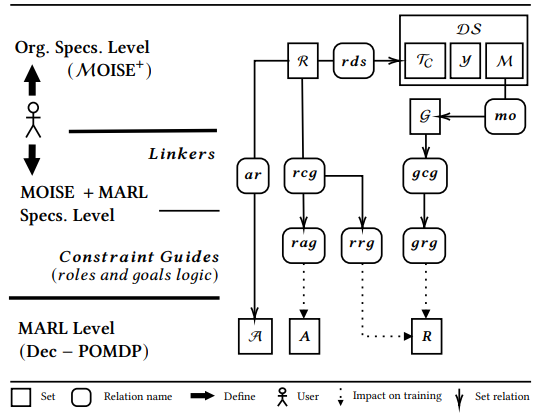
\includegraphics[width=0.6\linewidth]{figures/mm_simple_representation.png}
    \end{figure}
\end{frame}
    
\begin{frame}{Annexes}{Aperçu de PRAHOM}
    \begin{figure}
        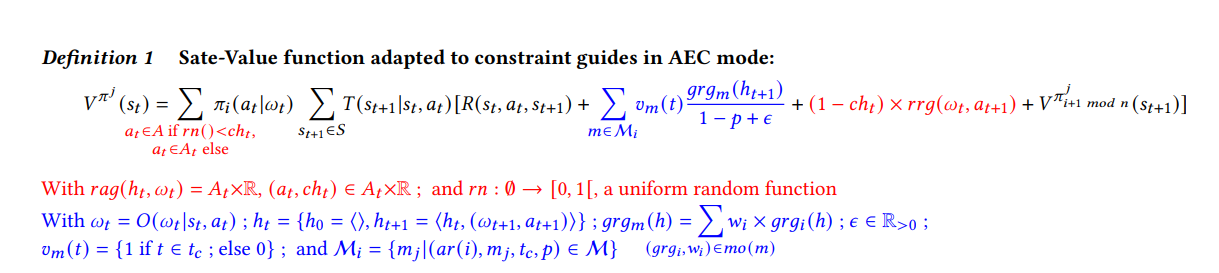
\includegraphics[width=\linewidth]{figures/modified_state_value_function.png}
    \end{figure}
\end{frame}
    
\begin{frame}[allowframebreaks]{Annexes}{Approche AOMEA : Fondement théorique}
    \textbf{Contraindre l'espace des politiques} pendant l'entraînement

    \begin{columns}
    
        \begin{column}{0.3\textwidth}
    
            \begin{itemize}
                \item À chaque étape, l'ensemble des actions disponibles est modifié pour correspondre aux contraintes de politiques définies par les utilisateurs ;
                \item Contraintes intégrées via : correction externe, apprentissage, modification interne des politiques.
            \end{itemize}
    
        \end{column}
    
        \begin{column}{0.8\textwidth}
            \begin{figure}
                \centering
                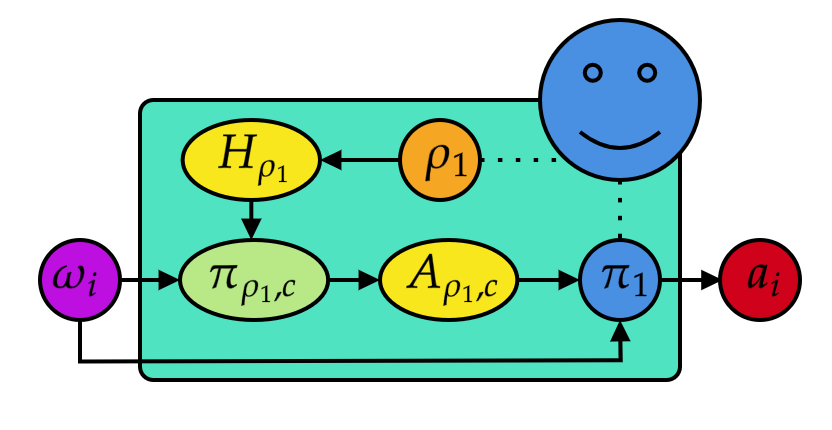
\includegraphics[width=0.7\linewidth]{figures/prahom_training_constrain.png}
                \caption*{Vue résumée de la contrainte PRAHOM}
                \label{fig:prahom_process}
            \end{figure}
        \end{column}
    
    \end{columns}
\end{frame}

\begin{frame}{Annexes}{Constrained Reinforcement Learning (Constrained-RL)}
    
    \begin{itemize}
        \item Apprendre une politique optimisant la récompense tout en respectant des \textbf{contraintes de sécurité} ou de \textbf{performance}.
        
        \item \textbf{Contraintes dures} : doivent toujours être respectées (Shielding).
        \item \textbf{Contraintes douces} : respectées en moyenne ou sous forme de pénalités.
        
        \item \textbf{Méthodes :}
            \begin{itemize}
                \item \textbf{Reward Shaping} : ajout de pénalités pour violation de contraintes.
                \item \textbf{Policy Projection} : ajustement des actions pour rester dans les limites.
                \item \textbf{Dual Variables} : intégration de multiplicateurs de Lagrange pour gérer les contraintes.
            \end{itemize}
            
    \end{itemize}    
\end{frame}

\begin{frame}{Annexes}{Safe Exploration et Shielding en Reinforcement Learning}
    
    \begin{itemize}
        \item \textbf{Safe Exploration} $\rightarrow$ garantir la sécurité lors de la phase d'exploration en limitant les risques de comportements dangereux.
        \item Principalement modifier la fonction de récompense (Langragien) pour integrer contraintes mais aussi\dots
        \item \textbf{Shielding} intervenir en temps réel pour bloquer les actions susceptibles de violer ces contraintes, permettant une exploration sécurisée.
    \end{itemize}
    
    \textbf{Référence :} \\
    \textit{Akifumi Wachi, Wataru Hashimoto, Xun Shen, \& Kazumune Hashimoto (2023). Safe Exploration in Reinforcement Learning: A Generalized Formulation and Algorithms. In Thirty-seventh Conference on Neural Information Processing Systems.}

\end{frame}

\begin{frame}[allowframebreaks]{Annexes}{Approche AOMEA: Fondement théorique}

    \textbf{Inferrer des Spécifications Organisationnelles}

    \begin{columns}

        \begin{column}{0.3\textwidth}

            \begin{itemize}
                \item \textbf{Knowledge-based Organizational Specifications Identification (KOSIA)}
                \item \textbf{General Organizational Specifications Infererence (GOSIA)}
            \end{itemize}

        \end{column}

        \begin{column}{0.8\textwidth}
            \begin{figure}
                \centering
                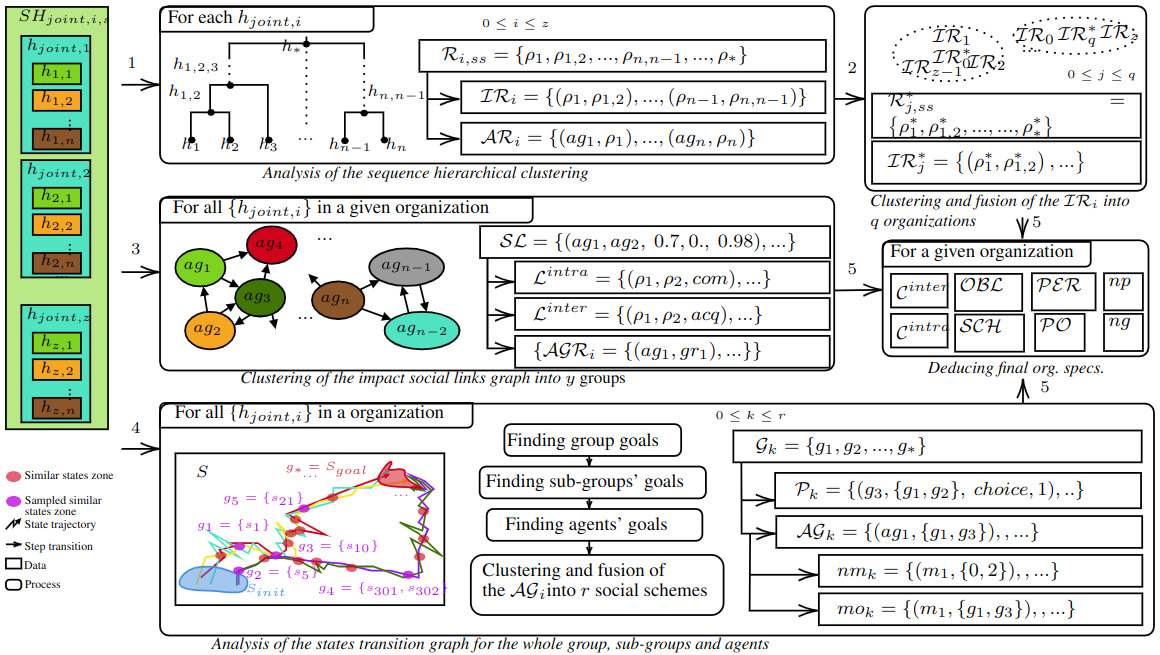
\includegraphics[width=0.95\linewidth]{figures/GOSIA_view.png}
                \caption*{A summary view of the GOSIA process}
                \label{fig:gosia_process}
            \end{figure}
        \end{column}

    \end{columns}

\end{frame}


%%%%%%%%%%%%%%%%

% Slide 2: Exemple d'utilisation
\begin{frame}[fragile]{Annexes}{Exemple d'utilisation d'Optuna}
    \begin{itemize}
        \item \textbf{Optuna} est une bibliothèque open-source pour l'optimisation des hyperparamètres (HPO), utile en apprentissage automatique.
        \item Exemples d'hyper-paramètre : taux d'apprentissage, fonction activation, nb couche, taille couches, seuil de ressemblance pour Hierarchical Clustering\dots
        \item \textbf{Étapes pour utiliser Optuna :}
        \begin{itemize}
            \item \texttt{1.} Définir une fonction d'objectif.
            \item \texttt{2.} Lancer une étude avec Optuna.
            \item \texttt{3.} Utiliser le meilleur résultat pour entraîner le modèle.
        \end{itemize}
    \end{itemize}

    \begin{lstlisting}[language=Python, basicstyle=\small\ttfamily, frame=single, caption=Exemple d'Optuna en Python]
import optuna

def objective(trial):
    x = trial.suggest_float("x", -10, 10)
    return (x - 2) ** 2 # Mock : fonction "etat-valeur"

study = optuna.create_study(direction="minimize")
study.optimize(objective, n_trials=100)

print(study.best_params)  # Affiche les meilleurs parametres
    \end{lstlisting}
\end{frame}


\begin{frame}{Annexes}{Aperçu PettingZoo}
    \begin{itemize}
        \item Bibliothèque Python pour environnements multi-agents.
        \item Simplifier l'entraînement et l'évaluation des agents dans divers environnements.
        \item \textbf{Caractéristiques principales} :
        \begin{itemize}
            \item Supporte plusieurs types d'environnements multi-agents (tour par tour, simultané, etc.).
            \item Intégration facile avec des frameworks de reinforcement learning comme RLlib.
            \item Compatible avec les API de Gym, permettant une utilisation intuitive.
        \end{itemize}
        \item \textbf{Exemples d'environnements inclus} :
        \begin{itemize}
            \item Jeux : \textit{TicTacToe}, \textit{ConnectFour}.
            \item Scénarios de collaboration et de compétition : \textit{Pistonball}, \textit{Prisoner's Dilemma}.
            \item Intégration avec la suite d'environnements Atari pour le multi-agent.
        \end{itemize}
    \end{itemize}
\end{frame}

\begin{frame}[fragile]{Annexes}{Exemple utilisation de PettingZoo}
    \begin{itemize}
        \item Exemple : Création et interaction avec un environnement.
        \item Chargement de l'environnement, réinitialisation et étapes d'interaction pour un agent.
    \end{itemize}
    \vspace{0.3cm}
    \begin{lstlisting}[language=Python, basicstyle=\ttfamily\small]
from pettingzoo.butterfly import pistonball_v6

# Creer et reinitialiser l'environnement
env = pistonball_v6.env()
env.reset()

# Boucle principale d'interaction
for agent in env.agent_iter():
    obs, reward, done, info = env.last()
    action = env.action_space(agent).sample()  # Action aleatoire
    env.step(action)
    if done:
        env.reset()  # Reinitialiser si l'episode est termine
\end{lstlisting}
\end{frame}


\begin{frame}{Annexes}{KB-Org}
    \frametitle{Organization-based multi-agent systems: From modeling to implementation}
    
    \begin{itemize}
        \item Modélisation et mise en œuvre des SMA basés sur organisation ;
        \item Intègre les concepts d'organisation pour structurer les interactions et le comportement des agents ;
        \item Banque d'organisations disponibles prêtes à être utilisé ;
        \item Explicabilité et à la coordination.
    \end{itemize}
    
    \

    Sims, V. (2008). Automated organization design for multi-agent systems. Autonomous Agents and Multi-Agent Systems, 16(2), 151-185.

\end{frame}

\begin{frame}{Annexes}{Présentation de la bibliothèque MARLlib}

    \begin{itemize}
        \item Bibliothèque Python pour MARL
        \item Supporte plusieurs environnements MARL comme PettingZoo, StarCraft II, MPE (Multi-Agent Particle Environment), etc.
        \item Implémente divers algorithmes MARL, incluant MADDPG, MAPPO, etc.
        \item Fournit une interface pour comparaison d’algorithmes, l’entraînement et l’évaluation.
        \item Offre des configurations \textit{fine-tunés} pour de nombreux environnements
    \end{itemize}

\end{frame}

\begin{frame}[allowframebreaks]{Annexes}{Présentation de la bibliothèque MARLlib}

    \begin{itemize}
        \item \textbf{Algorithmes Basés sur les Valeurs}  
        \begin{itemize}
            \item \textbf{Multi-Agent Q-Learning} : Une extension multi-agent fondamentale de Q-learning.  
            \textit{Description} : Simple à implémenter, mais avec des difficultés de scalabilité et de non-stationnarité.
            \item \textbf{MADDPG} : Une adaptation de DDPG pour les environnements multi-agents.  
            \textit{Description} : Gère bien les espaces d'actions continues, mais requiert beaucoup de données et est complexe.
        \end{itemize}
    
        \

        \item \textbf{Algorithmes Basés sur les Politiques}  
        \begin{itemize}
            \item \textbf{REINFORCE} : Une méthode de gradient de politique basique pour l'apprentissage direct de la politique.  
            \textit{Description} : Adaptable aux environnements stochastiques mais souffre de variances élevées des gradients.
            \item \textbf{Multi-Agent PPO (MAPPO)} : Une extension de PPO conçue pour les configurations multi-agents.  
            \textit{Description} : Stabilise les mises à jour, mais nécessite un ajustement minutieux et un coût de calcul élevé.
        \end{itemize}
    
        \item \textbf{Algorithmes Hybrides}  
        \begin{itemize}
            \item \textbf{A3C (Asynchronous Advantage Actor-Critic)} : Combine l'apprentissage des politiques et des valeurs pour un équilibre exploration/exploitation.  
            \textit{Description} : Accélère l'entraînement mais nécessite une synchronisation complexe.
            \item \textbf{MAPPO} : Un hybride intégrant PPO avec un entraînement centralisé.  
            \textit{Description} : Efficace pour les tâches coopératives, mais difficile dans les environnements compétitifs et exigeant en ressources.
        \end{itemize}
    
        \item \textbf{Algorithmes Théoriques et Coopératifs Basés sur le Jeu}  
        \begin{itemize}
            \item \textbf{Independent Q-Learning (IQL)} : Une version indépendante de Q-learning pour chaque agent.  
            \textit{Description} : Simple à implémenter mais avec de sérieux problèmes de non-stationnarité en multi-agent.
            \item \textbf{COMA (Counterfactual Multi-Agent Policy Gradients)} : Utilise des baselines contrefactuelles pour évaluer les contributions des agents.  
            \textit{Description} : Réduit la variance et améliore la coopération, mais demande des calculs lourds.
        \end{itemize}
    
        \item \textbf{Entraînement Centralisé avec Exécution Décentralisée}  
        \begin{itemize}
            \item \textbf{QMIX} : Décompose les valeurs Q pour améliorer la coordination multi-agent.  
            \textit{Description} : Équilibre l'entraînement centralisé et l'action décentralisée, mais moins efficace en environnements très compétitifs.
            \item \textbf{VDN (Value Decomposition Networks)} : Simplifie la coordination multi-agent avec la décomposition des valeurs.  
            \textit{Description} : Efficace mais limité dans la gestion d'interactions complexes.
        \end{itemize}
    \end{itemize}
    

\end{frame}


\end{document}
